\documentclass[../Cours.tex]{subfiles}

\begin{document}

\chapitre{Triangles}

\partie{Constructions}

\definition{Un triangle est une figure plane formée par 3 points et les segments qui les relient.}

\propriete{\centerline{\fbox{Inégalité triangulaire} \vspace{2ex}} Dans un triangle, la longueur d'un côté est toujours inférieure à la somme des longueurs des deux autres côtés.}

\exemple{
    \begin{figure}[!h]
        \centering
        \begin{tikzpicture}
            \coordinate (A) at (0,0);
            \coordinate (B) at (3,1);
            \coordinate (C) at (2,3);
            \draw (A) -- (B) -- (C) -- cycle;
            \node[below] at (A) {$A$};
            \node[below] at (B) {$B$};
            \node[above] at (C) {$C$};
            \node at (7,1+1) {$AB \leq AC + BC$};
            \node at (7,1.5) {$AC \leq AB + BC$};
            \node at (7,1) {$BC \leq AB + AC$};
        \end{tikzpicture}
        \caption{Exemple de triangle $ABC$}
    \end{figure}
}

\consequence{Si au moins une des inégalités n'est pas vraie, alors le triangle ne peut pas être construit.}

\propriete{Il suffit de vérifier l'inégalité correspondant au plus grand côté.}

\propriete{La somme des angles internes d'un triangle vaut \ang{180}.}

\clearpage
\partie{Les différents types de types de triangles et leurs propriétés}
\souspartie{Triangle rectangle}

\definition{Un triangle rectangle possède un angle droit (=\ang{90}).}

\begin{figure}[!h]
    \centering
    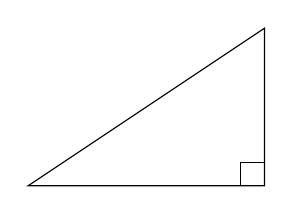
\begin{tikzpicture}
        \draw (0,0) -- (3,0) -- (3,2) -- cycle;
        \draw (3,0) rectangle (2.7,0.3);
    \end{tikzpicture}
\end{figure}


\souspartie{Triangle isocèle}

\definition{Un triangle isocèle possède deux côtés de même longueur.}
\vocabulaire{Le troisième côté est appelé la base du triangle.}
\propriete{Les angles à la base d'un triangle isocèle sont égaux.}

\begin{figure}[h!]
    \centering
    \begin{tikzpicture}
        \draw (0,0) -- (-2,-1) -- (2,-1) -- cycle;
        \node at (-1,-0.5) {||};
        \node at (1,-0.5) {||};
        \draw[fill=rouge,rouge] ($(-2,-1)+(0.5,0)$) arc (0:28:0.5) -- (-2,-1) -- cycle;
        \draw[fill=rouge,rouge] ($(2,-1)+(-0.5,0)$) arc (180:152:0.5) -- (2,-1) -- cycle;
    \end{tikzpicture} 
\end{figure}

\souspartie{Triangle équilatéral}

\definition{Un triangle équilatéral a ses trois côtés de même longueur.}
\propriete{Les trois angles intérieurs sont chacun égaux à \ang{60}.}

\begin{figure}[h!]
    \centering
    \begin{tikzpicture}
        \draw (0,0) -- ($({3*cos(60)},{3*sin(60)})$) -- (3,0) -- cycle;
    \end{tikzpicture}
\end{figure}

\partie{Droites remarquables dans un triangle}

\souspartie{Médiatrices}

\definition{La médiatrice d'un segment est la droite qui coupe le segment en son milieu perpendiculairement.}

\remarque{Dans un triangle, il y a 3 médiatrices.}

\propriete{Les trois médiatrices d'un triangle concourent en un point appelé le centre du cercle circonscrit.}

\consequence{Dans un triangle $ABC$, si $M$ est le centre du cercle circonscrit : $$MA = MB = MC$$}

\souspartie{Hauteurs}

\definition{Dans un triangle, la hauteur d'un côté est la droite perpendiculaire à ce côté et qui passe par le segment opposé.}

\notation{Dans un triangle $ABC$, la hauteur du côté $[AB]$ se nomme aussi la hauteur issue de $C$.}

\propriete{Les trois hauteurs d'un triangle concourent en un point : l'orthocentre.}

\clearpage

\renewcommand\tabularxcolumn[1]{m{#1}}
\begin{tabularx}{\textwidth}{C|C}\hline
    \makecell{La hauteur du côté $[AB]$ \\ la hauteur issue de $C$} & 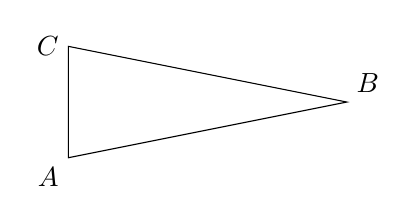
\begin{tikzpicture}[rotate=-45]
        \coordinate (A) at (0,0);
        \coordinate (B) at (2,3);
        \coordinate (C) at (-1,1);
        \draw (A) node[below left]{$A$} -- (B) node[above right]{$B$} -- (C) node[left]{$C$} -- cycle;
    \end{tikzpicture} \\\hline
    .... & \begin{tikzpicture}[rotate=-35]
        \coordinate (A) at (0,0);
        \coordinate (B) at (2,3);
        \coordinate (C) at (-1,1);
        \draw (A) node[below left]{$A$} -- (B) node[above right]{$B$} -- (C) node[left]{$C$} -- cycle;
        \coordinate (H) at ($(B)!(A)!(C)$);
        \draw[dashed] ($(A)!-0.2!(H)$) -- ($(A)!1.5!(H)$);
    \end{tikzpicture} \\\hline
    .... & \begin{tikzpicture}[rotate=-35]
        \coordinate (A) at (0,0);
        \coordinate (B) at (3,2);
        \coordinate (C) at (-1,1);
        \draw (A) node[below left]{$A$} -- (B) node[above right]{$B$} -- (C) node[left]{$C$} -- cycle;
        \coordinate (I) at ($(B)!0.5!(C)$);
        \coordinate (v) at (1,-4);
        \draw[dashed] ($(I)-0.5*(v)$) -- ($(I)+0.5*(v)$);
    \end{tikzpicture} \\\hline
    La médiatrice de $[AC]$ & 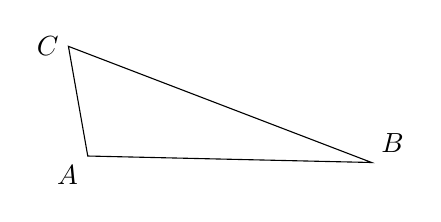
\begin{tikzpicture}[rotate=-35]
        \coordinate (A) at (0,0);
        \coordinate (B) at (3,2);
        \coordinate (C) at (-1,1);
        \draw (A) node[below left]{$A$} -- (B) node[above right]{$B$} -- (C) node[left]{$C$} -- cycle;
    \end{tikzpicture} \\\hline
    Les trois médiatrices de $ABC$ & \begin{tikzpicture}[rotate=-25]
        \coordinate (A) at (0,-1);
        \coordinate (B) at (3,1.5);
        \coordinate (C) at (-1,0);
        \draw (A) node[below left]{$A$} -- (B) node[above right]{$B$} -- (C) node[left]{$C$} -- cycle;
        \coordinate (I) at ($(B)!0.5!(C)$);
        \coordinate (v) at (1.5,-4);
        \draw[dashed] ($(I)-0.5*(v)$) -- ($(I)+0.5*(v)$);
    \end{tikzpicture} \\\hline
    Les trois hauteurs de $ABC$ & \begin{tikzpicture}[rotate=-25]
        \coordinate (A) at (-0.6,-1.8);
        \coordinate (B) at (3,1.5);
        \coordinate (C) at (-2,0);
        \draw (A) node[below left]{$A$} -- (B) node[above right]{$B$} -- (C) node[left]{$C$} -- cycle;
        \coordinate (H) at ($(B)!(A)!(C)$);
        \draw[dashed] ($(A)!-0.2!(H)$) -- ($(A)!1.5!(H)$);
    \end{tikzpicture} \\\hline
\end{tabularx}

\end{document}